\subsection{Matrix Factorization Models} \label{bg:sub:factorizationmodels}
%Function
MF methods are dimensionality reduction techniques used for recommendation that generally find latent features for items, and the propensity for users towards each latent feature. This helps with finding nontrivial correlations in the data as a latent feature could be something that is not at all obvious, but is really important.

A sparse dataset, such as a rating matrix with many items and users, with most cells being zero, we face the \textit{curse of dimensionality}. It is harder to find similar users, because the many dimensions makes differences bigger. Consider a user who has 100 ratings on movies as opposed to 5 ratings on genres. In machine learning, dimensionality reduction concerns itself with mapping these original 100 ratings to a lower dimensional space, such as that of ratings of genres, although these new dimensions are not explicitly known. These are the aforementioned latent features, that now describe each item, rather than the explicitly known features of the original high dimension dataset\cite{preprocessing}.

MF makes an approximation of a matrix of ratings by decomposing it into multiple matrices. Since MF approximates matrices in an offline step before recommendation, it scales better compared to contemporary collective filtering techniques during recommendation, as most of the calculation work has been done offline. It performs well even when data sparsity is a concern due to the matrix approximation and the dimensionality reduction.
As data sparsity grows in a set, the less accurate every method gets. Factorization methods counteract this by compressing the data, making it less sparse, and easier to cluster.
As an MF matrix is traditionally updated offline resulting in unchanging matrices, the matrix can be reused as required. This is a benefit when testing various aggregations or configurations of users as most of the calculations are already done as part of the training of the matrix. As the part can be reused for all the tests, it can save some time in practice.

\subsubsection{Singular Value Decomposition}
On its own, SVD is a dimensionality reduction technique. However, in 2006 Simon Funk popularized it as a recommender method with some modifications\footnote{Source: http://sifter.org/~simon/journal/20061211.html}\cite{svdsimonfunk}.

Given a matrix of user ratings, SVD works by decomposing the matrix as seen in Equation \ref{eq:svd_decomp} into two matrices called the left and right singular vectors, $U$ and $V$ respectively, and a matrix holding the nonzero singular values on its diagonal, $\Sigma$, as per the SVD theorem\cite{svdtheorem}. For this example, the left singular vector would hold the users on one side, and their inclination towards each latent feature. The right vector would conversely hold all the rated items, and their inclination towards each latent feature\cite{linearalgebra_svd}\cite{preprocessing}. 

\begin{equation} \label{eq:svd_decomp}
\centering
R = U\times \Sigma \times V^T
\end{equation}

SVD considers as many features as there are ranks, but not all of them are influential. Reducing the number of features to consider is trivial, as the largest singular values stored in $\Sigma$ have the most influence and are sorted by size.

At this point, it is possible to find some interesting similarities among the users, however to use SVD for recommendation, we must account for the missing ratings. By slightly tweaking the equation, as seen in Equation \ref{eq:svd_AB_squeezing}, we get an $A$ and $B$ matrix, holding users and items respectively. This results in three matrices looking like Figure \ref{fig:svdSqueeze}, where $F$ is the number of latent features, throughout the report $F$ and $f$ will be used interchangeably. 

\begin{equation}\label{eq:svd_AB_squeezing}
\centering
U\times \Sigma \times V^T = U\Sigma^{1/2} \Sigma^{1/2}V^T = AB
\end{equation}

The $A$ and $B$ matrices can give us our rating matrix, as can be seen in Equation \ref{eq:svd_R}, before the training starts. After the $A$ and $B$ matrices have been trained, which will be described in next section, this is how the prediction matrix $\hat{R}$ is found.

\begin{equation}\label{eq:svd_R}
\centering
R = AB
\end{equation}

\begin{figure}[H]
	\centering
	\includegraphics[scale=0.8]{svd_ab_squeeze.png}
	\caption{The decomposition of a rating matrix using SVD\cite{preprocessing}}
	\label{fig:svdSqueeze}
\end{figure}
Moving to the dense subspace of each rated item and user being defined by their features rather than their explicit ratings, data sparsity becomes less of a problem, as missing ratings are squeezed out, as they are subsumed into the lower dimensions for the items.

Equation \ref{eq:svd_num_decomp} is an example of a decomposition of a 3-by-3 matrix into 3 matrices as per Equation \ref{eq:svd_decomp}, the result being the left singular vector, eigenvalues, and right singular vector respectively. Note that the eigenvalues are sorted such that each eigenvalue is smaller.
\footnotesize
\begin{equation}\label{eq:svd_num_decomp}
\centering
\begin{bmatrix}
1 & 0 & 4\\ 
0 & 2 & 5\\ 
3 & 0 & 6
\end{bmatrix} = 
\begin{bmatrix}
-0.44 & 0.08 	& -0.89 \\ 
-0.54 & -0.82 	& 0.2	\\ 
-0.71 & 0.57 	& 0.41
\end{bmatrix} \times 
\begin{bmatrix}
9.2 & 0		& 0		\\ 
0 	& 2.45	& 0		\\ 
0 	& 0		& 0.53
\end{bmatrix} \times
\begin{bmatrix}
   -0.28 &   0.73  &  0.62 \\
   -0.12 &  -0.67  &  0.74 \\
   -0.95 &  -0.13  & -0.27
\end{bmatrix}
\end{equation}
\normalsize
In Equation \ref{eq:svd_AB_num_squeezing}, the decomposition is split into an $A$ and $B$ matrix as seen in Equation \ref{eq:svd_AB_squeezing}. Note that the square root of the eigenvalues matrix appears in both calculations.
\footnotesize
\begin{equation}\label{eq:svd_AB_num_squeezing}
\begin{split}
A = \begin{bmatrix}
-0.44 & 0.08 	& -0.89 \\ 
-0.54 & -0.82 	& 0.2	\\ 
-0.71 & 0.57 	& 0.41
\end{bmatrix} \times 
\begin{bmatrix}
9.2 & 0		& 0		\\ 
0 	& 2.45	& 0		\\ 
0 	& 0		& 0.53
\end{bmatrix}^{\frac{1}{2}} =
\begin{bmatrix}
   -1.35 &   0.13 &  -0.65 \\
   -1.65 &  -1.28 &   0.14 \\
   -2.16 &   0.9  &   0.3
\end{bmatrix}
\\
B = \begin{bmatrix}
9.2 & 0		& 0		\\ 
0 	& 2.45	& 0		\\ 
0 	& 0		& 0.53
\end{bmatrix}^{\frac{1}{2}} \times
\begin{bmatrix}
   -0.28 &   0.73  &  0.62 \\
   -0.12 &  -0.67  &  0.74 \\
   -0.95 &  -0.13  & -0.27
\end{bmatrix} =
\begin{bmatrix}
   -0.85 &  -0.36 &  -2.89 \\
    1.15 &  -1.04 &  -0.21 \\
    0.45 &   0.54 &  -0.2
\end{bmatrix}
\end{split}
\end{equation}
\normalsize

It is then possible to reconstruct the rating matrix $R$ and in time, after the training, the prediction matrix $\hat{R}$, using the approach shown in Equation \ref{eq:svd_R}. An example of this can be seen in Equation \ref{eq:svd_R_example}.
\footnotesize
\begin{equation}\label{eq:svd_R_example}
R = \begin{bmatrix}
   -1.35 &   0.13 &  -0.65 \\
   -1.65 &  -1.28 &   0.14 \\
   -2.16 &   0.9  &   0.3
\end{bmatrix} \times
\begin{bmatrix}
   -0.85 &  -0.36 &  -2.89 \\
    1.15 &  -1.04 &  -0.21 \\
    0.45 &   0.54 &  -0.2
\end{bmatrix} = 
\begin{bmatrix}
1 & 0 & 4\\ 
0 & 2 & 5\\ 
3 & 0 & 6
\end{bmatrix}
\end{equation}
\normalsize
\subsubsection{Gradient Descent}
In Funk's blog, the gradient descent optimization algorithm is proposed as a common method to learn the A and B matrices to minimize the error, as found using Equation \ref{eq:gradient_descent_error}. The error is calculated as the euclidean distance between our known ratings, $R$, and our predicted ratings $\hat{R}$\cite{aibook_gradientdescent_localsearch}.

\begin{equation}\label{eq:gradient_descent_error}
\text{Error} = |R-\hat{R}| = |R - AB| = \sum_{u=1}^{U}\sum_{i=1}^{I}\left (R_{ui}- \sum_{f=1}^{F} A_{uf}B_{fi} \right )^2
\end{equation}

Given as a function, the gradient will point in the direction of the largest error increase, as shown in Equation \ref{eq:derivative_gradient}. So to minimize the error, steps are taken towards the negative of the gradient\cite{aibook_gradientdescent_linearfunc}.

\begin{equation}\label{eq:derivative_gradient}
	\begin{split}
	\frac{dError}{dA}=-(R-AB)B^T = \sum_{i=1}^{I}(R_{ui} - \sum_{n=1}^{N} A_{un}B_{ni})B_{fi}
	\\
	\frac{dError}{dB}=-(R-AB)A^T = \sum_{u=1}^{U}(R_{ui} - \sum_{n=1}^{N} A_{un}B_{ni})A_{uf}
	\end{split}
\end{equation}

Taking the average error when finding the derivative is a costly operation for learning the A and B matrices, as it sums up the error for every user-item pair across all of their features. This can be expressed by the running time $\Theta(U\times I \times F)$.

The common solution is using the stochastic gradient descent. For this, a single observed rating is selected at random for each update step of the gradient descent, rather than summing up over all the item-user pairs to find the exact gradient. The updates will be a bit more erratic than seen in Figure \ref{fig:gradientDescent}\footnote{Source: https://en.wikipedia.org/wiki/Gradient\_descent\label{ftn:wikifigure}}, but will overall converge towards a local minimum.

\begin{figure}
	\centering
	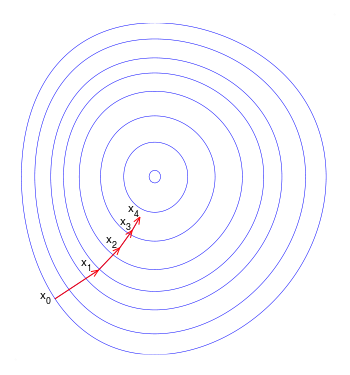
\includegraphics[scale=0.5]{gradientdescent.png}
	\caption{Gradient descent showing steps as it converges toward a local minimum\footref{ftn:wikifigure}}
	\label{fig:gradientDescent}
\end{figure}

The learning rate describes the speed at which the error is corrected at each step. A high learning rate results in fewer steps and a lower chance of getting stuck in a local minimum, however a high learning rate makes convergence more difficult as the model can end up dancing around the minimum by taking too large steps near the end. A too small learning rate can result in the model settling in a local minimum for the cost function, unable to escape, as the gradient of the error will always point back towards the nearest local minimum and is slow to train. A learning rate is usually between $0.1$ and $0.001$, but it is recommended to take an exploratory approach. In Equation \ref{eq:matrixfactorization_learningrate}, $\eta$ is the learning rate.

\begin{equation}\label{eq:matrixfactorization_learningrate}
	\begin{split}
	A_{uf}\leftarrow A_{uf} + \eta(R_{ui}-\sum_{n=1}^{N}A_{un}B_{ni})B_{fi}
	\\
	B_{fi}\leftarrow B_{fi} + \eta(R_{ui}-\sum_{n=1}^{N}A_{un}B_{ni})A_{uf}
	\end{split}
\end{equation}

Regularization helps avoid overfitting, where a model fits its training data too closely so that it predicts extremely well but only within the training data. It is added as an additional modifier when updating the model as can be seen in Equation \ref{eq:matrixfactorization_regularization}, where $\lambda$ is the regularization value. It makes the resulting model more general, which improves accuracy when moving beyond the training set.

\begin{equation}\label{eq:matrixfactorization_regularization}
	\begin{split}
	A_{uf}\leftarrow A_{uf} + \eta(R_{ui}-\sum_{n=1}^{N}A_{un}B_{ni})B_{fi}-\lambda A_{uf}
	\\
	B_{fi}\leftarrow B_{fi} + \eta(R_{ui}-\sum_{n=1}^{N}A_{un}B_{ni})A_{uf} -\lambda B_{fi}
	\end{split}
\end{equation}

After the $A$ and $B$ matrices have been trained it is possible to construct a prediction 

%http://www.kyb.mpg.de/fileadmin/user_upload/files/publications/attachments/CFEMF_KDDW2007_4614[0].pdf